\chapter[Traffic flow]{Traffic flow\\[0.5cm] Linear cascades\\ Linear systems\\
Delay differential equations\\ Laplace transform}
\label{chap:traffic_flow}



\section{An ODE model of traffic flow}

We want to model a situation with $N$ cars on a straight road with no overtaking, and where a given driver adjusts (instantaneously) their speed on the speed the driver in front of them.
\subsection{Hypotheses}
\begin{itemize}
\item $N$ cars in total,
\item the road is the $x$-axis,
\item $x_n(t)$ is the position of the $n$th car at time $t$,
\item $v_n(t)\stackrel{\Delta}{=}x_n'(t)$ is the velocity of the $n$th car at time $t$,
\item all cars start with the same initial speed $v_0$ at time $t=0$.
\end{itemize}
\begin{figure}[htbp]
\begin{center}
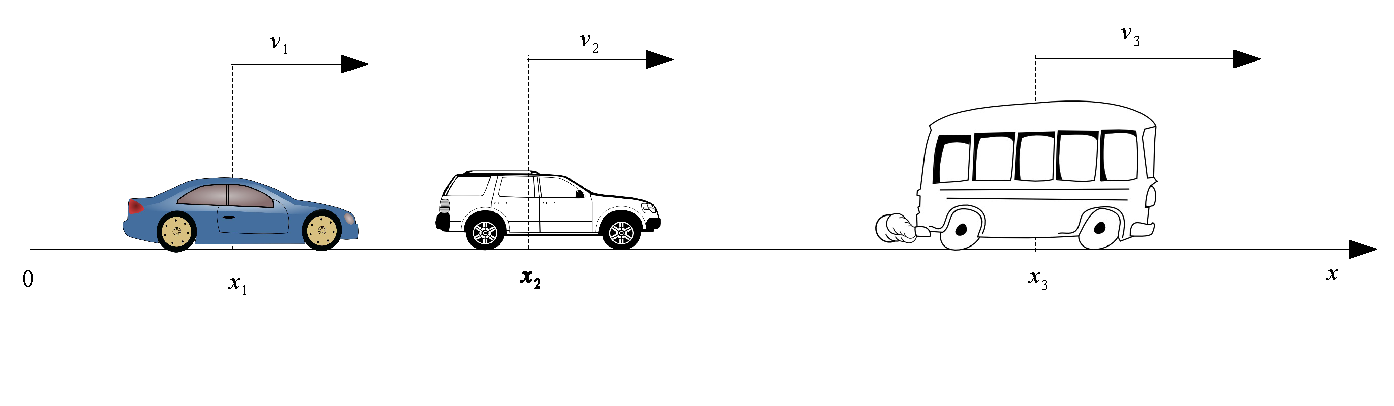
\includegraphics[width=0.8\textwidth]{../figs_06_traffic_flow/traffic_flow1}
\caption{The situation described by the model of traffic flow.}
\label{fig:traffic_flow_ODEmodel}
\end{center}
\end{figure}
To make computations easier, we express the velocity of cars in a reference frame
moving at the speed $u_0$. (Remark that here, speed and velocity are equal, since movement is 1-dimensional.)
Let
\[
u_n(t)=v_n(t)-u_0.
\]
Then $u_n(t)=0$ for $t\leq 0$, and $u_n$ is the speed of the $n$th car in the moving frame coordinates.


\subsection{Modeling driver behavior}
Assume that a driver adjusts their speed according to relative speed between their car and the car in front, and that this adjustment is a linear term, equal to $\lambda$ for all drivers. This implies the following.
\begin{itemize}
\item
For the first car, the evolution of speed remains to be determined.
\item 
For the second car,
\[
u_2'=\lambda(u_1-u_2).
\]
This means that if the speed of the second car, $u_2$, is larger than that of the first car, $u_1$, then the driver of the second car decreases their speed ($u_2'$ has a negative sign). Similarly, if the speed of the second car is smaller than that of the first car, then the term $\lambda(u_2-u_1)$ is positive, implying that $u_2'>0$, i.e., the second car speeds up.
\item
Similarly, the third car adjusts its speeds as a function of the car in front, i.e., car number 2, giving
\[
u_3'=\lambda(u_2-u_3).
\]
\item 
Thus, for $n=1,\ldots,N-1$,
\begin{equation}\label{eq:ode_traffic_flow}
u_{n+1}'=\lambda(u_n-u_{n+1}).
\end{equation}
\end{itemize}

\subsection{Solving using linear cascades}
This can be solved using \emph{linear cascades}: if $u_1(t)$ is known, then
\[
u_2'=\lambda(u_1(t)-u_2)
\]
is a linear first-order nonhomogeneous equation. The solution (obtained using integrating factors or variation of constants) is
\[
u_2(t)=\lambda e^{-\lambda t}\int_0^t u_1(s)e^{\lambda s}ds.
\]
Then use this function $u_2(t)$ in $u_3'$ to get $u_3(t)$,
\begin{align*}
u_3(t) &= \lambda e^{-\lambda t}\int_0^t u_2(s)e^{\lambda s}ds.
\end{align*}
Thus
\begin{align*}
u_3(t) &= \lambda e^{-\lambda t}\int_0^t u_2(s)e^{\lambda s}ds \\
&= \lambda e^{-\lambda t}\int_0^t 
\left(\lambda e^{-\lambda s}\int_0^s u_1(q)e^{\lambda q}dq\right)ds \\
&= \lambda^3 e^{-\lambda t}\int_0^t e^{-\lambda s}\int_0^s u_1(q)e^{\lambda q}dqds.
\end{align*}
Continue the process to get the solution.

\subsection{An example with known first driver behavior}
Suppose that the driver of car 1 follows the function
\[
u_1(t)=\alpha\sin(\omega t),
\]
that is, $\omega$-periodic, 0 at $t=0$ (we want all cars to start with speed relative to the moving reference frame equal to 0), and with amplitude $\alpha$.
Then
\begin{align*}
u_2(t) &= \lambda\alpha e^{-\lambda t}\int_0^t \sin(\omega s)e^{\lambda s}ds \\
&= \lambda\alpha e^{-\lambda t}
\left(
\frac{\omega-\omega e^{\lambda t} \cos(\omega t)+\lambda e^{\lambda t} \sin(\omega t)}{\lambda^2+\omega^2}
\right) \\
&= \frac{\lambda\alpha}{\lambda^2+\omega^2}\left(\omega e^{-\lambda t}
+\lambda\sin(\omega t)-\omega\cos(\omega t)\right).
\end{align*}
When $t\to\infty$, the first term goes to 0 and we are left with a $\omega$-periodic
term.
Continuing the process,
\[
u_3(t) = \frac{\lambda^2\alpha}{\lambda^2+\omega^2} e^{-\lambda t}
\int_0^t \left(\omega e^{-\lambda s}
+\lambda\sin(\omega s)-\omega\cos(\omega s)\right)e^{\lambda s}ds,
\]
that is,
\begin{align*}
u_3(t) &= \frac{\lambda^2\alpha}{\lambda^2+\omega^2}e^{-\lambda t}\left(\omega t+\int_0^t \left(\lambda\sin(\omega s)-\omega\cos(\omega s)\right)e^{\lambda s}ds\right) \\
&= \frac{\lambda^2\alpha}{\lambda^2+\omega^2}\left(\omega t+\frac{2 \lambda \omega}{\lambda^2+\omega^2}\right)e^{-\lambda t}\\
&\quad -\frac{\lambda^2\alpha}{(\lambda^2+\omega^2)^2}\left(2 \lambda \omega \cos(\omega t)-\lambda^2 \sin(\omega t)+\omega^2 \sin(\omega t)\right).
\end{align*}
Once again, the terms in $e^{-\lambda t}$ vanishes for large $t$, and we are left with 3 $\omega$-periodic terms.




\section{Linear systems -- Our case}
\subsection{General computations, case of 3 cars}
We consider the case of 3 cars. Let
\[
X=\begin{pmatrix}
u_2\\ u_3
\end{pmatrix}
\]
Then the system can be written as
\[
X'=\begin{pmatrix}
-\lambda & 0 \\
\lambda & -\lambda
\end{pmatrix}X
+\begin{pmatrix}
\lambda u_1(t)\\ 0
\end{pmatrix}
\]
which we write for short as $X'=AX+B(t)$.
The matrix $A$ has the eigenvalue $-\lambda$ with multiplicity 2. Its Jordan form can be obtained using the maple function {\tt JordanForm}:
\begin{verbatim}
> with(LinearAlgebra)
> A := <<-lambda, lambda> | <0, -lambda>>:
> J := JordanForm(A)
\end{verbatim}
giving
\[
J=\begin{pmatrix}
-\lambda & 1 \\
0 & -\lambda
\end{pmatrix}
\]
To get the matrix of change of basis, 
\begin{verbatim}
> P := JordanForm(A,output='Q')
\end{verbatim}
giving
\[
P=\begin{pmatrix}
0 & 1 \\
\lambda & 0
\end{pmatrix}
\]
which is such that $P^{-1}AP=J$.
Because $-\lambda$ is an eigenvalue with multiplicity 2 (the same multiplicity as as the size of the matrix), we can use the simplified theorem Theorem~\ref{th:Jordan_simple_case}, and only need $N$. 
We have
\begin{align*}
N &= A-S \\
&=\begin{pmatrix}
-\lambda & 0 \\
\lambda & -\lambda
\end{pmatrix}
-
\begin{pmatrix}
-\lambda & 0 \\
0 & -\lambda
\end{pmatrix} \\
&=\begin{pmatrix}
0 & 0 \\
\lambda & 0
\end{pmatrix}.
\end{align*}
Clearly, $N^2=0$, so, by the theorem in the simplified case,
\begin{align*}
x(t) &= e^{-\lambda t}\left(\II+Nt\right)x_0 \\
\end{align*}
But we know that solutions are unique, and that the solution to the differential equation is given by $x(t)=e^{At}x_0$. This means that
\begin{align*}
e^{At} &= e^{-\lambda t}\left(\II+Nt\right)\\
&= e^{-\lambda t}\left(\begin{pmatrix}1&0\\0&1\end{pmatrix}+
\begin{pmatrix}
0 & 0 \\
\lambda t & 0
\end{pmatrix}\right)\\
&= e^{-\lambda t}\begin{pmatrix}
1 & 0 \\
\lambda t & 1
\end{pmatrix} \\
&= \begin{pmatrix}
e^{-\lambda t} & 0 \\
\lambda te^{-\lambda t} & e^{-\lambda t}
\end{pmatrix}.
\end{align*}
Now notice that the solution to
\[
X'=AX
\]
is trivially established here, since
\[
X(0)=\begin{pmatrix}u_2(0)\\u_3(0)\end{pmatrix}=\begin{pmatrix}0\\0\end{pmatrix},
\]
and thus
\[
X(t)=e^{At}0=0.
\]
The matrix $e^{At}$ does however play a role in the solution (fortunately), since it is involved in the variation of constants formula:
\[
X(t)=e^{At}X_0+\int_0^t e^{A(t-s)}B(s)ds.
\]
Thus we need to compute $e^{A(t-s)}B(s)$, and then the integral.
\begin{align*}
e^{A(t-s)}B(s) &= 
\begin{pmatrix}
e^{-\lambda (t-s)} & 0 \\
\lambda (t-s)e^{-\lambda (t-s)} & e^{-\lambda (t-s)}
\end{pmatrix}
\begin{pmatrix}
\lambda u_1(s)\\ 0
\end{pmatrix} \\
&= \begin{pmatrix}
\lambda e^{-\lambda(t-s)}u_1(s) \\
\lambda^2e^{-\lambda(t-s)} (t-s)u_1(s)
\end{pmatrix}
\end{align*}
and thus
\begin{align*}
\int_0^t e^{A(t-s)}B(s)ds &=
\int_0^t\left(
\begin{array}{ll}
\lambda e^{-\lambda(t-s)}u_1(s) \\
\lambda^2e^{-\lambda(t-s)} (t-s)u_1(s)
\end{array}
\right)ds \\
&= \left(\begin{array}{ll}
\int_0^t\lambda e^{-\lambda(t-s)}u_1(s) ds \\
\int_0^t\lambda^2e^{-\lambda(t-s)} (t-s)u_1(s) ds
\end{array}
\right) \\
&= \left(\begin{array}{ll}
\lambda e^{-\lambda t} \int_0^te^{\lambda s}u_1(s) ds \\
\lambda^2 e^{-\lambda t}\int_0^te^{\lambda s} (t-s)u_1(s) ds
\end{array}
\right) \\
&= \left(\begin{array}{ll}
\lambda e^{-\lambda t} \int_0^te^{\lambda s}u_1(s) ds \\
\lambda^2 e^{-\lambda t}\left(t\int_0^te^{\lambda s}u_1(s) ds
-\int_0^tse^{\lambda s} u_1(s) ds\right)
\end{array}
\right).
\end{align*}
Let
\[
\Psi(t)=\int_0^t e^{\lambda s} u_1(s)ds
\]
and
\[
\Phi(t)=\int_0^t se^{\lambda s} u_1(s)ds.
\]
These can be computed when we choose a function $u_1(t)$. Then, finally, we have
\begin{align*}
X(t) &= \int_0^t e^{A(t-s)}B(s)ds \\
&= \left(\begin{array}{ll}
\lambda e^{-\lambda t} \Psi(t) \\
\lambda^2 e^{-\lambda t}\left(t\Psi(t)
-\Phi(t)\right)
\end{array}
\right).
\end{align*}


\subsection{Specialization to the case of the $\alpha\sin(\omega t)$ driver}
We set
\[
u_1(t)=\alpha\sin(\omega t).
\]
Then
\begin{align*}
\Psi(t) &= \frac{\alpha (\omega-\omega e^{\lambda t} \cos(\omega t)+\lambda e^{\lambda t} \sin(\omega t))}{\lambda^2+\omega^2}
\end{align*}
and
\begin{align*}
\Phi(t) =\frac{\alpha(\lambda^3 t+\lambda t \omega^2-\lambda^2+\omega^2) \sin(\omega t) e^{\lambda t}}{(\lambda^2+\omega^2)^2}
-\frac{\alpha\omega \cos(\omega t) (t \lambda^2+t \omega^2-2 \lambda) e^{\lambda t}+2\alpha \lambda \omega}{(\lambda^2+\omega^2)^2}
\end{align*}


\begin{figure}[htbp]
\begin{center}
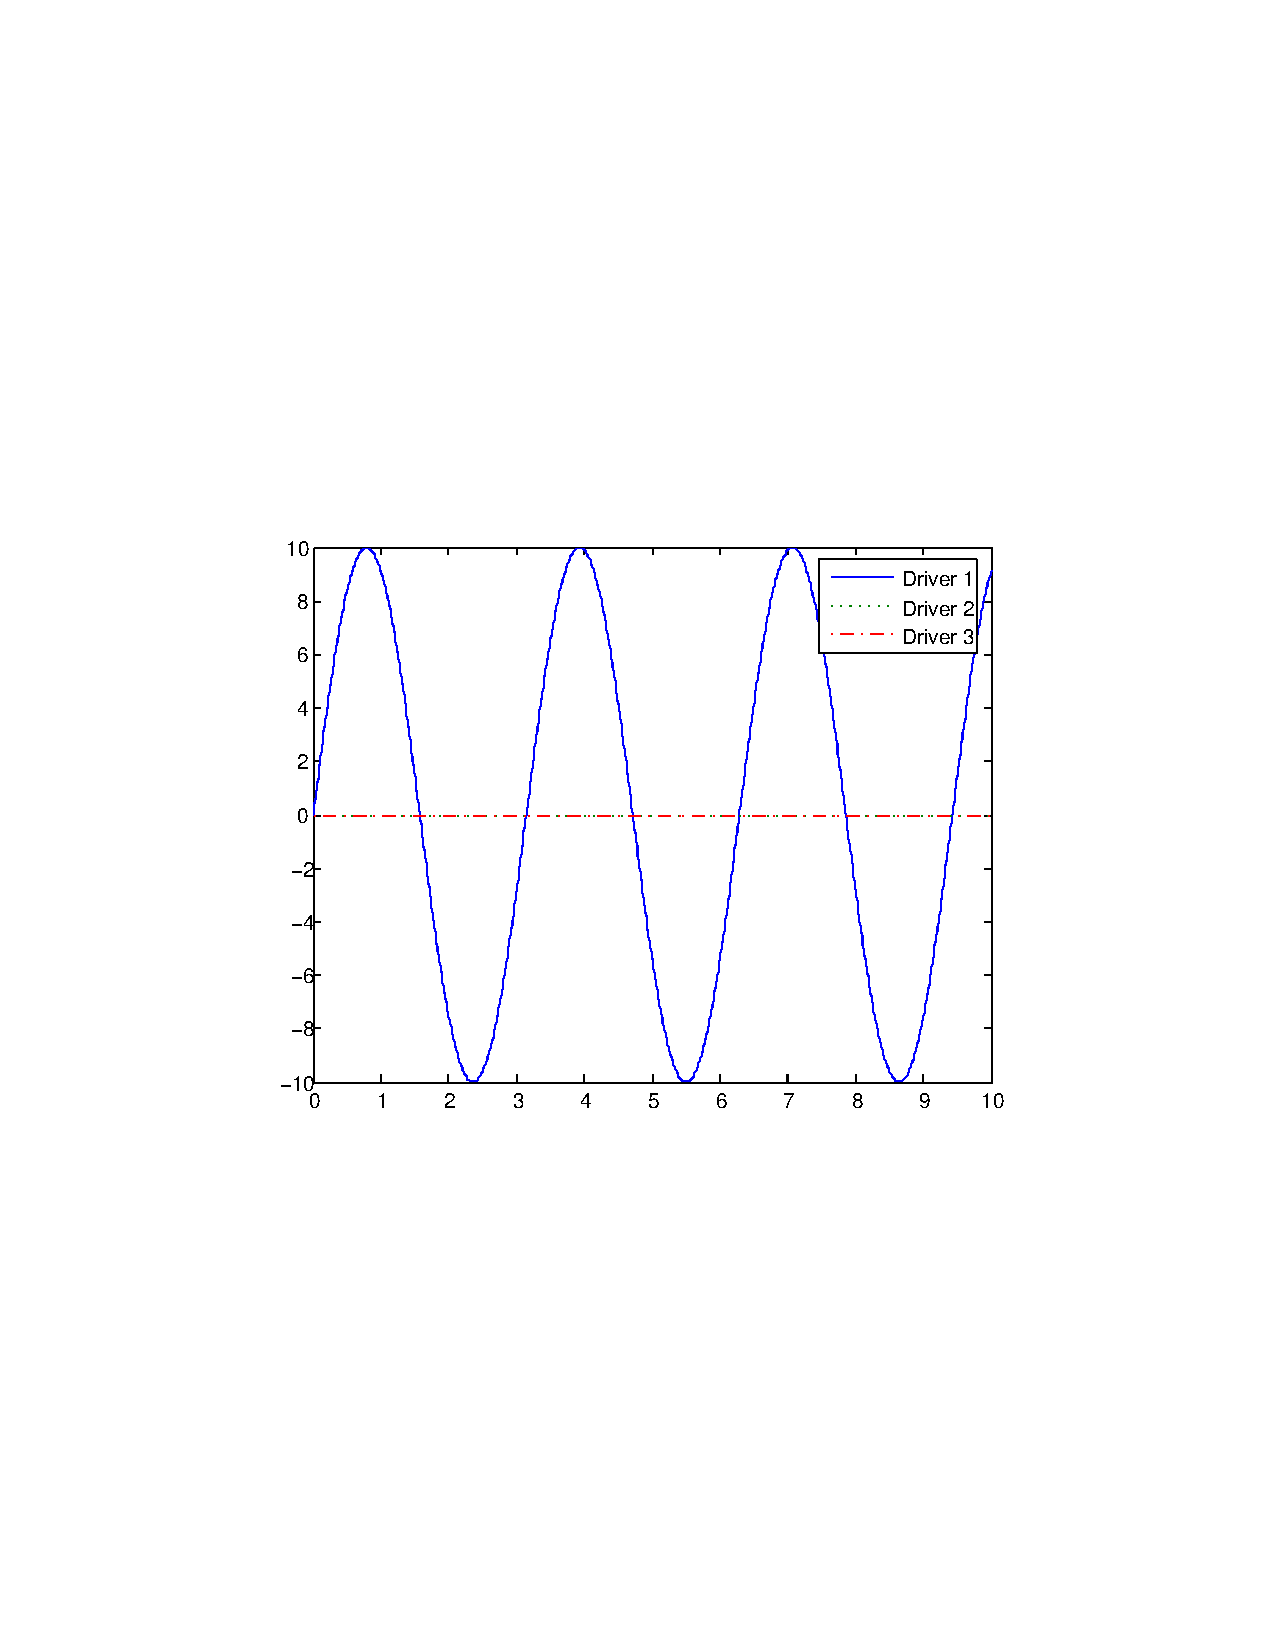
\includegraphics[width=0.49\textwidth]{../figs_06_traffic_flow/traffic_flow_3cars_ODE_l0}
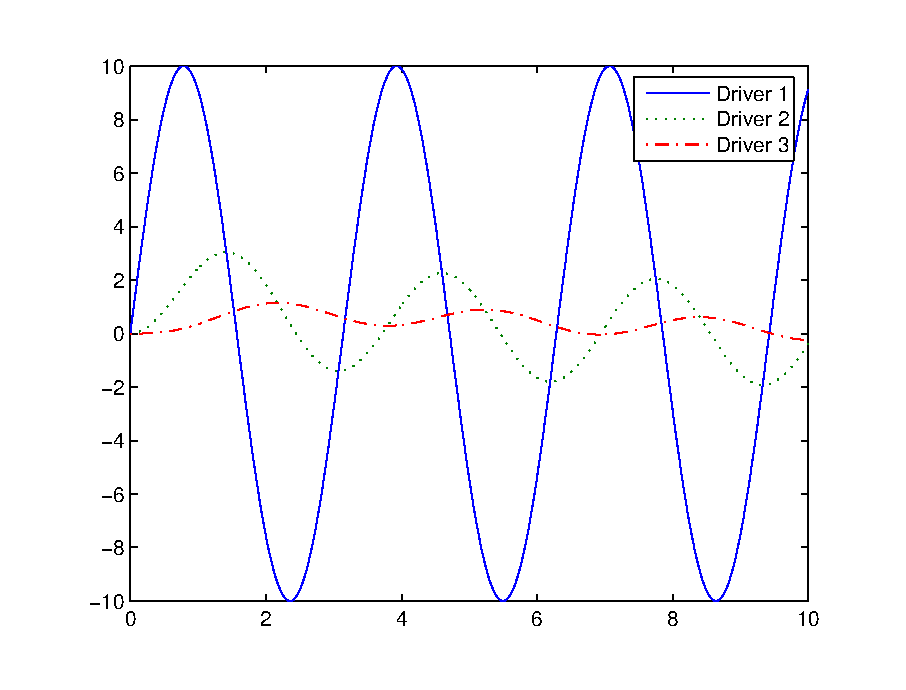
\includegraphics[width=0.49\textwidth]{../figs_06_traffic_flow/traffic_flow_3cars_ODE_l04}
\end{center}
\caption{$\lambda=0$ (left)and $\lambda=0.4$ (right).}
\end{figure}

\begin{figure}[htbp]
\begin{center}
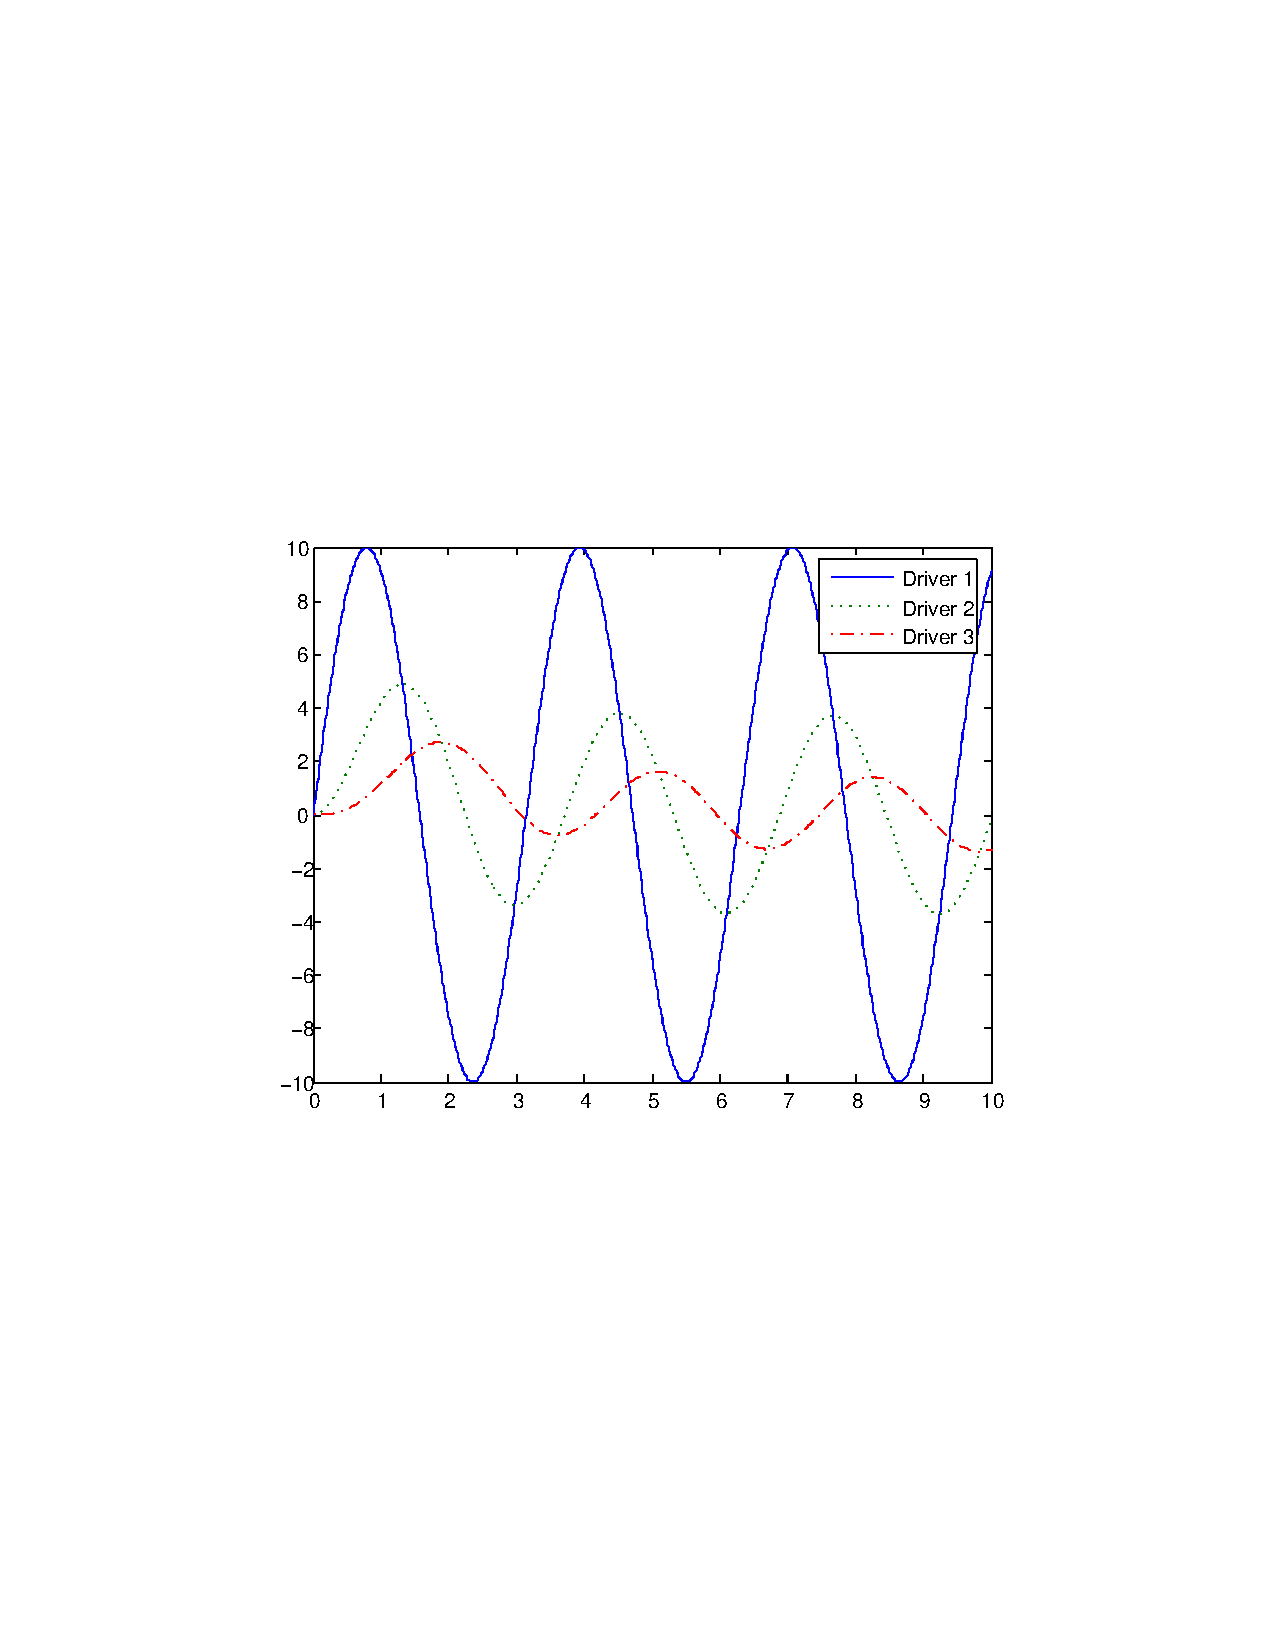
\includegraphics[width=0.49\textwidth]{../figs_06_traffic_flow/traffic_flow_3cars_ODE_l08}
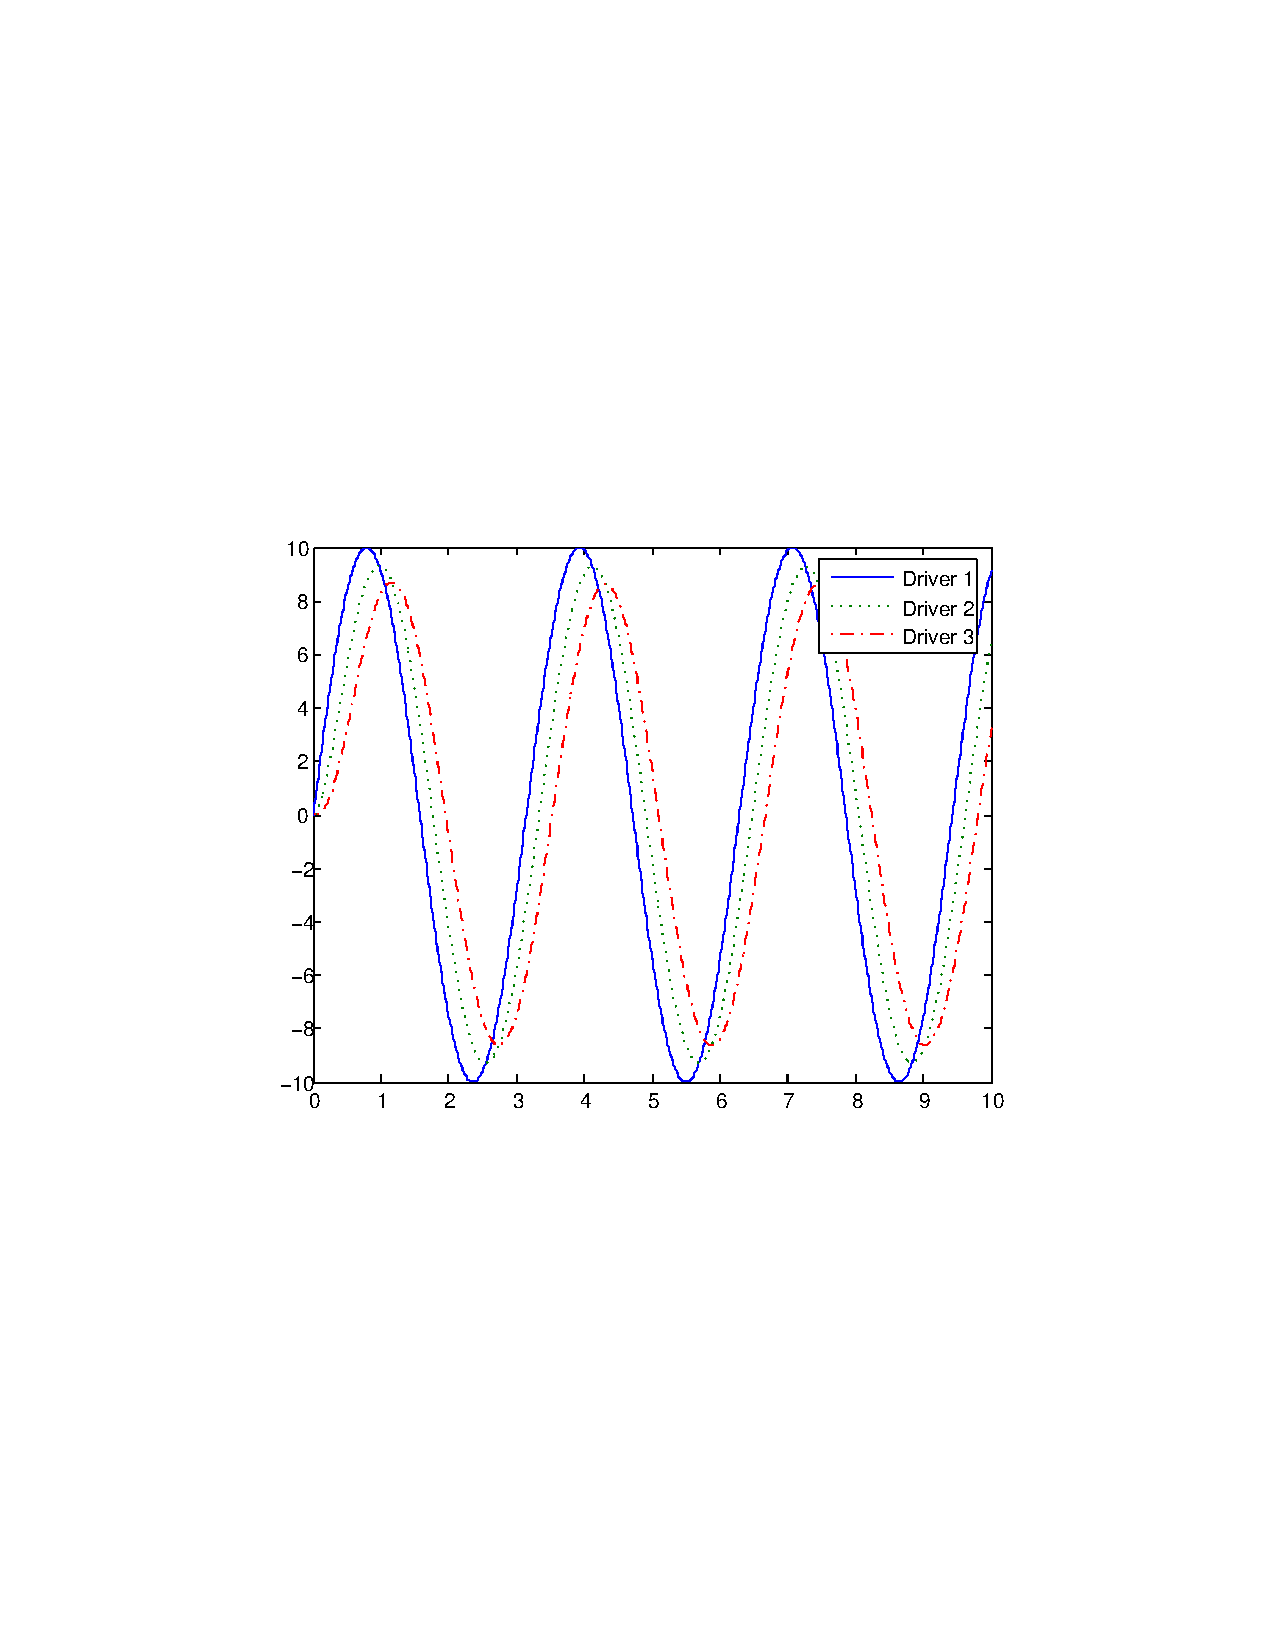
\includegraphics[width=0.49\textwidth]{../figs_06_traffic_flow/traffic_flow_3cars_ODE_l5}
\end{center}
\caption{$\lambda=0.8$ (left) and $\lambda=5$ (right).}
\end{figure}





















\section{Prey-Predator model}
{\bf 1 prey:}


$x(t)$ is the density of prey, and $y(t)$ is the density of predators
$$
\begin{array}{lll}
\frac{dx}{dt}&=x(r-\frac{r}{K}x -ay)&r,K,a >0\\
\frac{dy}{dt}&=y(-b+cx)& b,c>0
\end{array}
$$
\begin{itemize}
\item $ay$ is the per capita loss of prey to the predator.
\item $cx$ is the per capita gain to the predator.
\end{itemize}


{\bf 2 preys:}
\begin{itemize}
\item $x$ is the predator, it dies out in the absence of prey
\item $y$ is a prey, it grows exponentially in the absence of predators
\item $z$ is a prey, it grows logistically in the absence of predators
\end{itemize}


$$
\begin{array}{cl}
\frac{dx}{dt}=&\alpha xz+\beta xy -\gamma x\\
\frac{dy}{dt}=&\delta y-\epsilon xy\\
\frac{dz}{dt}=&\mu z(\nu-z) - \chi xz
\end{array}
$$

Equlibria:
$$(0,0,0) \quad and \quad (\frac{\delta}{\epsilon},\frac{1}{\beta}(\gamma -\alpha \nu +\frac{\alpha\chi\delta}{\epsilon \mu}),\nu-\frac{\delta \chi}{\epsilon \mu})$$



\section{Growth of living organisms}
\subsection{Michaelis-Menten enzyme kinetics}
Michaelis Menten dynamics: $e$ enzyme concentration, $s$ subtrate concentration, $c$ complexe concentration, $p$ product concentration
\begin{align*}
\frac{ds}{dt}=&-k_1se+k_{-1}c\\
\frac{de}{dt}=&-k_1se+k_{-1}c+k_2c\\
\frac{dc}{dt}=&k_1se-k_{-1}c-k_2c\\
\frac{dp}{dt}=&k_2c
\end{align*}
\begin{itemize}
\item quasi-equilibrium hypothesis ($\dfrac{dc}{dt}=0$) is valid when enzymes are efficient  $e_0<<s_0$ (small concentration of enzymes in comparison to concentration of substrate). 
\item velocity of reaction $\dfrac{dp}{dt}=K_{max}\dfrac{s}{k_n+s}$, uptake in nutrient ($\dfrac{dS}{dt}=-K_{max}\dfrac{s}{k_n+s}$ where $K_{max}=k_2e_0$ and $k_n=\frac{k_{-1}+k_2}{k_1}$), 
\item cooperative enzymes, Hill equation (generalization for n-subtrate complexes, $\dfrac{ds}{dt}=-K_{max}\dfrac{s^n}{k_n+s^n}$)
\end{itemize}
\subsubsection{Chemostat model}
\begin{figure}[h]
%\includegraphics[width=1\textwidth]{figs_steph/MM}
\caption{Cell with unbounded transmembranar receptor $x_0$, bounded transmembranar receptors $x_1$. Nutrient $n$ and $p$ product.}
\end{figure}
\begin{itemize}
\item Michaelis-Menten dynamics can be used to describe the growth of bacteria from a given uptake of substrate.
\item Inflow and outflow at a constant rate $D$ to keep a constant volume in the chemostat with a concentration $n_0$ of subtrate in the inflow.
\end{itemize}
\subsection{Kinetic reactions}
Autocatalysis
\subsection{Bifurcation}
\begin{itemize}
\item Saddle-node bifurcation:
$$\frac{dx}{dt}=\mu  - x^2$$
\item Transcritical bifurcation:
$$\frac{dx}{dt}=\mu x - x^2$$
\item Pitchfork bifurcation:
$$\frac{dx}{dt}=\mu x - x^3$$
\end{itemize}

%An irreversible reaction in which reactants $A$ and $B$ produce $C$:
%$$A+B\rightarrow C$$
%where $k$ is the reaction constant.
%
%We are interested in the dynamics of the product $C$
%\subsection{Host-Parasites}
%\subsection{Genetic model}
%\subsection{Physiology}
